\section{Introduction}
\label{sec1:Intro}

\IEEEPARstart{T}{he} development of autonomous agents capable of reasoning, planning, and executing complex tasks within dynamic environments remains a paramount objective in artificial intelligence. Central to this pursuit is the paradigm of World Models~\cite{ha2018world, hafner2019dream}, internal predictive engines that empower agents to forecast the spatiotemporal consequences of their actions before physical interaction. Contemporary theoretical frameworks~\cite{lecun2022path} posit that a robust world model serves as the cognitive substrate for intelligent systems. It facilitates learning from sparse rewards and enables planning over extended horizons by synthesizing potential future trajectories~\cite{hafner2020dreamerv2, hafner2023dreamerv3}. Consequently, constructing world models that simultaneously achieve high perceptual fidelity, strict spatiotemporal consistency, and precise action-controllability has emerged as a critical imperative across the computer vision and robotics communities~\cite{bruce2024genie, wu2024ivideogpt, wang2025sampo}.

Despite substantial advancements, visual world modeling remains bifurcated into two dominant paradigms, each with distinct theoretical merits and inherent limitations. The first, \textbf{Discrete Autoregressive Modeling}~\cite{van2017neural, esser2021taming}, formulates video generation as a sequence modeling task over quantized latent tokens. By discretizing continuous visual signals into finite codebook indices via mechanisms like VQ-VAE~\cite{van2017neural} or VQGAN~\cite{esser2021taming}, these frameworks leverage the powerful causal reasoning capabilities of transformers~\cite{vaswani2017attention, brown2020language} to predict future states sequentially~\cite{yan2021videogpt, rakhimov2020latent}. While highly effective at capturing macro-level semantic structures and maintaining causal consistency, this approach is fundamentally hindered by a quantization bottleneck. The discrete nature of finite codebooks imposes an intrinsic ceiling on visual fidelity, which frequently manifests as temporal flickering, the degradation of fine-grained textures, and an inability to model continuous physical dynamics (\textit{e.g.}, fluid turbulence or subtle illumination gradients)~\cite{yu2023magvit, yu2023language}. Furthermore, scaling the codebook capacity to mitigate these artifacts incurs prohibitive computational overhead.

%%%%%%%%%%%%%%%%%%
\IEEEpubidadjcol 
%%%%%%%%%%%%%%%%%%

Conversely, the second paradigm comprises \textbf{Continuous Generative Models}, notably Diffusion Probabilistic Models (DPMs)~\cite{ho2020denoising, rombach2022high} and emerging Flow Matching architectures~\cite{lipman2023flow, liuflow}. Operating directly within continuous latent manifolds, these methodologies successfully circumvent quantization errors, thereby achieving state-of-the-art perceptual quality~\cite{peebles2023scalable, liu2024sora, blattmann2023stable}. Nevertheless, they often lack the explicit, structured reasoning capabilities demanded by long-horizon planning. Standard continuous generative architectures frequently fail to preserve object permanence and temporal coherence during extended rollouts, primarily because they lack the strong causal inductive biases inherent to autoregressive systems. Furthermore, embedding precise action-conditional control into these continuous spaces remains a non-trivial challenge; naive concatenation of action vectors typically proves insufficient for effectively modulating the fine-grained kinematic dynamics of the generated scenes~\cite{zhang2023adding, mou2024t2i}.

\begin{figure*}
    \centering
    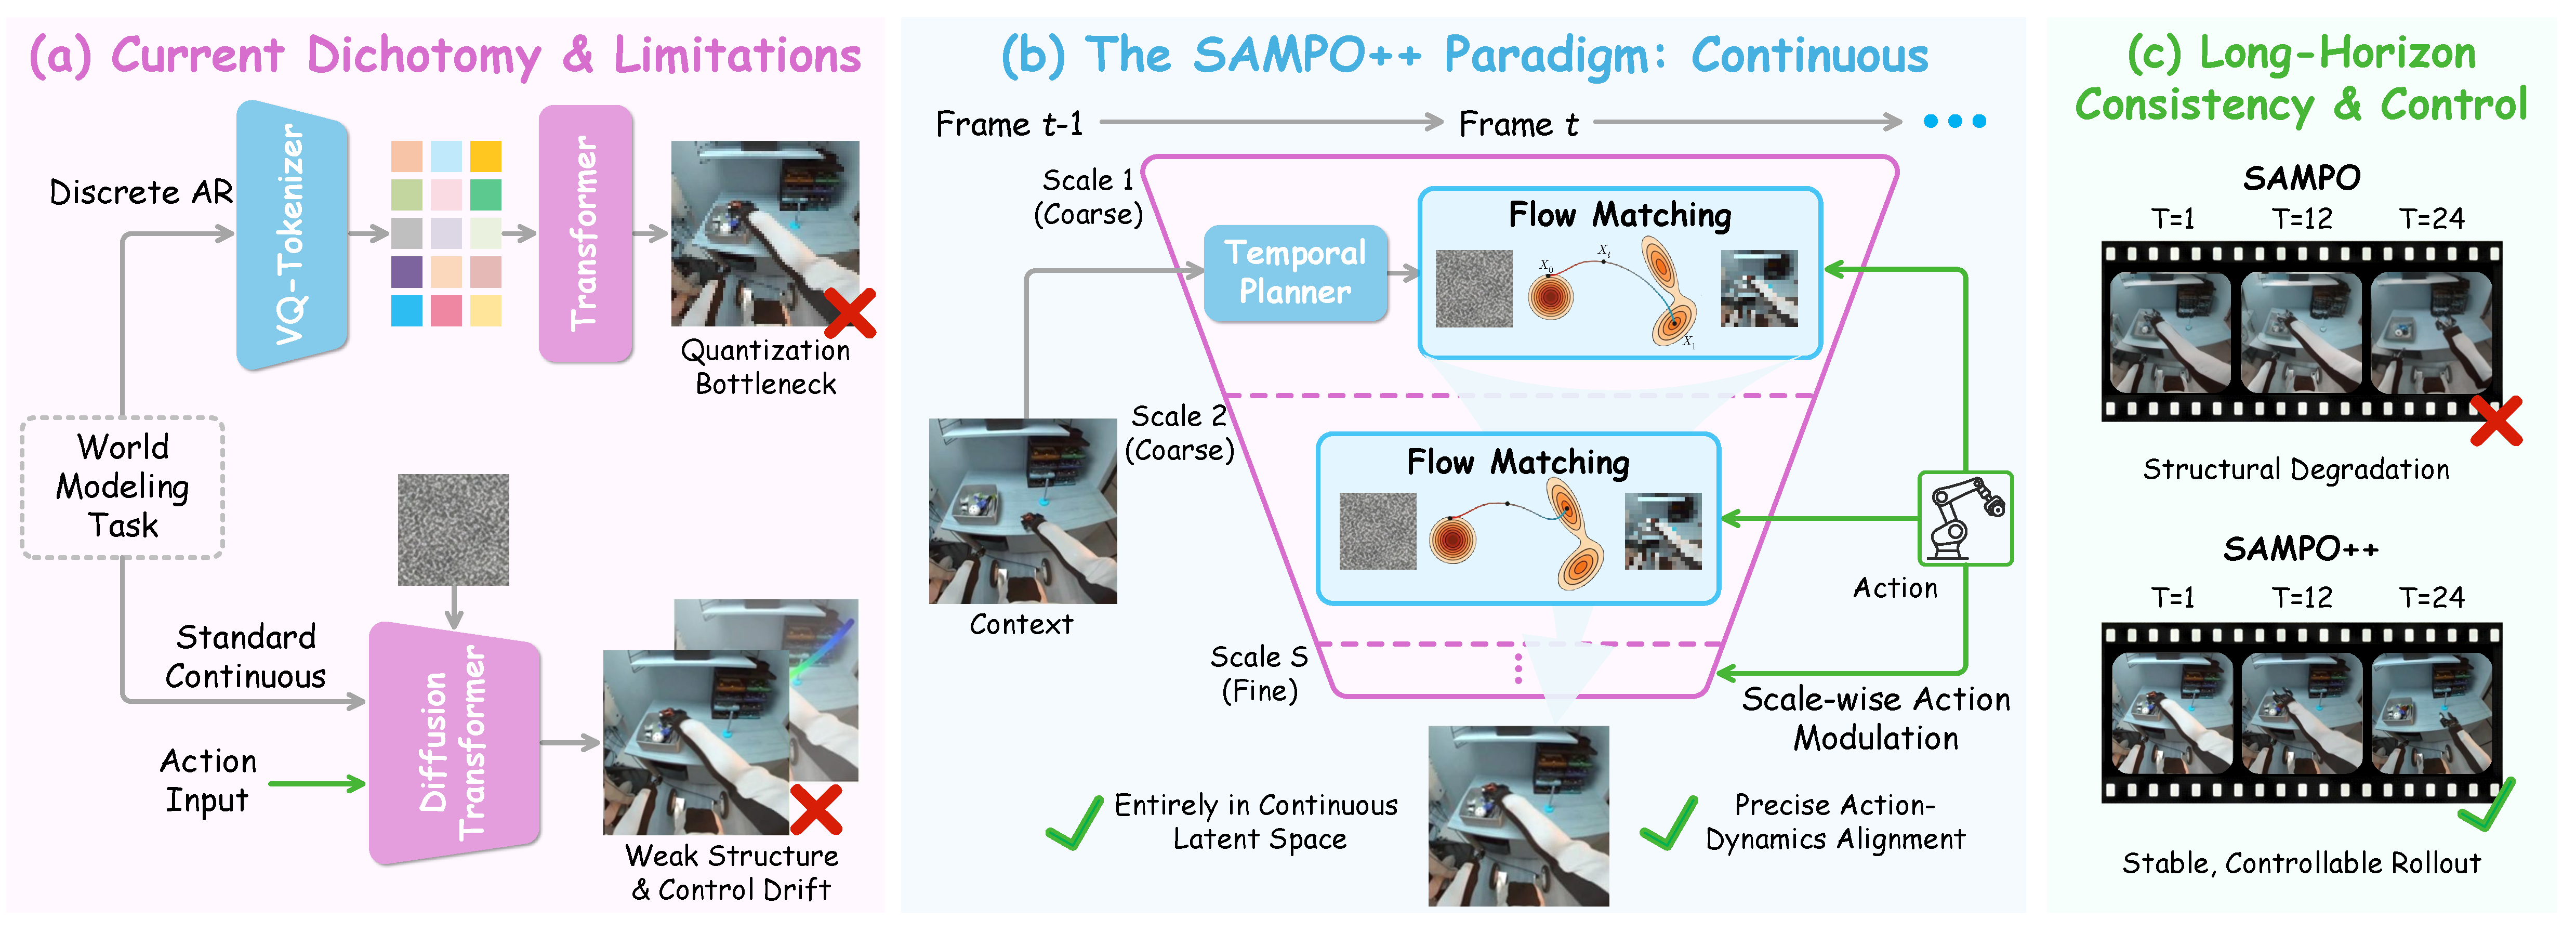
\includegraphics[width=\linewidth]{fig/fig1.pdf}
    \caption{\textbf{Conceptual comparison and framework overview.} 
    \textbf{(a) The prevailing dichotomy:} Existing world models confront a structural trade-off: discrete AR models are hindered by intrinsic quantization artifacts, whereas standard continuous models are restricted to fixed-length synthesis, thereby precluding interactive long-horizon generation.
    \textbf{(b) The SAMPO++ solution:} Our framework resolves this dilemma via a unified ``Predict-then-Refine'' paradigm, synergizing temporal autoregression with scale-wise flow matching directly on a continuous latent manifold. Crucially, it integrates Action-adaptive Dynamics Modulation to enforce precise, frequency-aware control.
    \textbf{(c) Performance:} Consequently, SAMPO++ demonstrates superior long-term physical coherence and action fidelity, effectively mitigating the degradation observed in state-of-the-art baselines.}   
    \label{fig1}
\end{figure*}

As illustrated in Figure~\ref{fig1}\textcolor{blue}{(a)}, this work postulates that the prevailing dichotomy between discrete causal reasoning and continuous high-fidelity generation constitutes a structural constraint rather than a fundamental theoretical limitation. We hypothesize that the hierarchical advantages of scale-wise progression, as demonstrated in recent frameworks~\cite{wang2025sampo,tian2024visual,li2024autoregressive}, can be fully preserved while systematically transcending the representational restrictions inherent to discrete tokenization.
To actualize this conceptual synergy, we propose SAMPO++ (see Figure~\ref{fig1}\textcolor{blue}{(b)}), a unified world modeling framework that seamlessly integrates temporal autoregressive modeling with scale-wise flow matching. Diverging from prior discrete approaches constrained by token indices, SAMPO++ operates entirely within a continuous latent manifold. The video generation process is formulated as a ``Predict-then-Refine'' paradigm: a temporal autoregressive backbone first predicts the coarse conditional distribution, establishing a robust structural prior. Subsequently, a scale-wise flow matching generator~\cite{ren2024flowar, ma2024sit} progressively synthesizes continuous latent features from noise based on this prior. This hybrid architecture effectively synergizes the long-horizon planning capabilities of autoregressive transformers with the resolution-independent synthesis potential of continuous flow matching.

Realizing this unified architecture entails three core technical innovations:

First, to realize unified scale-wise generative modeling, we replace the conventional ``next-token prediction'' objective with a next-scale flow conditional prediction objective. This formulation enables the synthesis of environmental dynamics in a coarse-to-fine manner, prioritizing global motion dynamics before resolving high-frequency textural details. This hierarchical approach effectively incorporates the inductive bias of human perception regarding macro-to-micro visual processing~\cite{denton2015deep}, thereby avoiding the quantization artifacts inherent in discrete modeling.

Second, to achieve precise action-controllability, we introduce an Action-adaptive Dynamics Modulation (ADM) mechanism, effectively overcoming the limitation where existing methods treat action inputs merely as passive conditions. Inspired by advances in pixel-space diffusion~\cite{yu2025pixeldit}, this module injects control signals via scale-aware affine transformations that modulate the feature statistics (mean and variance) of the flow matching layers~\cite{park2019spade, karras2019stylegan2}. Crucially, this modulation is disentangled across scales, allowing actions to distinctly influence global displacements at coarse scales and local deformations at fine scales, yielding a granularity of control previously unattainable.

Third, to ensure long-term spatiotemporal consistency and mitigate the compounding error accumulation inherent to continuous autoregression, we propose a Scale-Aware spacetime Rotary Position Embedding (SA-RoPE). This mechanism establishes a unified 4D positional encoding integrating time, space, and scale dimensions, thereby enforcing strict resolution hierarchy constraints during temporal evolution~\cite{su2024roformer,tian2025pdfactor,yesiltepe2025infinity}. Furthermore, we incorporate an inference-time flow trajectory rectification strategy that leverages optical flow priors to actively rectify latent feature drift and ensure rigorous physical consistency over extended horizons~\cite{teed2020raft, ji2026videoar}.

% To this end, we introduce SAMPO++, a unified world modeling framework integrating temporal autoregression with scale-wise flow matching within a fully continuous latent space. Formulated under a ``Predict-then-Refine'' paradigm, our architecture reconciles structured causal planning with high-fidelity continuous synthesis, thereby circumventing the quantization bottlenecks inherent to prior discrete approaches. 
Extensive empirical validation demonstrates that SAMPO++ establishes a new state-of-the-art across a broad spectrum of dynamic environments. Crucially, not only does our framework achieve unprecedented fidelity in passive video synthesis spanning robotic manipulation (\textit{e.g.}, BAIR~\cite{ebert2017selfBAIR}, RoboNet~\cite{dasari2019robonet}, 1X World Model~\cite{1X_Technologies_1X_World_Model_2024}) and autonomous driving (\textit{e.g.}, Cityscapes~\cite{Cityscapes}, OpenDV-YouTube~\cite{yang2024genad}), but it also serves as a highly reliable neural simulator for downstream control. Specifically, SAMPO++ sets new benchmarks in visual planning with action-conditioned rollouts on the VP$^2$ suite~\cite{tian2023control} and significantly elevates sample efficiency in model-based reinforcement learning (MBRL) within the complex Meta-World environments~\cite{yu2020meta}.
In summary, our main contributions are:
\begin{itemize}
    \item We propose SAMPO++, a unified world modeling architecture that bridges temporal autoregression with scale-wise flow matching, eliminating quantization artifacts while preserving robust causal planning capabilities.
    
    \item We design an Action-adaptive Dynamics Modulation (ADM) mechanism. By dynamically modulating generative flow statistics via scale-aware affine transformations, we achieve precise responsiveness.
        
    \item We introduce a Scale-Aware spacetime RoPE and a predictive flow rectification strategy, solving the degradation problem in long-horizon continuous video prediction.
    
    \item We provide a rigorous evaluation on five large-scale benchmarks covering indoor robotics and outdoor driving scenarios, setting new performance records and validating the scalability of the proposed approach.
\end{itemize}

%%%%%%%%%%%%%%%%%%%%%%%%%%%%%%%%%%%%%%%%%%%%%%%%%%%%%%%%%%%%%%%%%%%%%%%%%%
This paper substantially extends our preliminary conference version~\cite{wang2025sampo} and makes the following new contributions:
\begin{itemize}
    \item Proposing SAMPO++, a unified continuous-space framework merging temporal autoregression with scale-wise flow matching to bypass quantization bottlenecks for high-fidelity synthesis.
    
    \item Introducing Action-adaptive Dynamics Modulation, enabling precise controllability by injecting action signals into flow statistics via scale-aware affine transformations.
    
    \item Integrating Scale-Aware spacetime Rotary Position Embeddings and flow trajectory rectification to enforce long-term physical coherence using spatiotemporal-scale coordinates and optical flow priors.

    \item Conducting additional experiments on Cityscapes~\cite{Cityscapes} and OpenDV dataset~\cite{yang2024genad} and new ablation studies to validate the effectiveness of each component.
\end{itemize}

The remainder of this paper is organized as follows: Section~\ref{Sec2:RelatedWork} reviews related work on generative modeling paradigms and embodied world models. Section~\ref{Sec3:Method} details the proposed unified framework. Section~\ref{Sec4:Experiments} presents comprehensive experimental results and ablation studies. Finally, Section~\ref{Sec5:Conclusion} concludes the paper.

